\part{微分几何学}
\chapter{微分流形与李群基础}
\section{微分流形期末考试内容}
\subsection{证明题}
\begin{exam}
    证明 $n$ 维球面 $S^n=\{(x_1,\cdots,x_{n+1})\in\mathbb{R}^{n+1}\mid \sum_{i=1}^{n+1}x^2_i=1\}$ 是 $n$维 $C^\infty$ 微分流形.
\end{exam}
\begin{proof}
    取 $S^n$ 的拓扑为 $\R^{n+1}$ 子空间的拓扑, 则 $S^n$ 是Hausdorff空间.令
    \begin{equation}
        \begin{aligned}
            U^+_i &=\{(x_1,\cdots,x_{n+1})\in S^n\mid x_i>0\};\\
            U^-_i &=\{(x_1,\cdots,x_{n+1})\in S^n\mid x_i<0\}.\\
            \varphi_i^+ &\colon U_i^+ \to \R^n ,(x_1,\cdots,x_{n+1}) \to (x_1,\cdots,\hat{x_i},\cdots,x_{n+1});\\
            \varphi_i^- &\colon U_i^- \to \R^n ,(x_1,\cdots,x_{n+1}) \to (x_1,\cdots,\hat{x_i},\cdots,x_{n+1});
        \end{aligned}
    \end{equation}
    其中 $i=1,2,\cdots,n+1$,则 $\varphi_i^+$ 与 $\varphi_i^-$ 都是可逆映射,有
    \begin{equation*}
        \begin{aligned}
            (\varphi_i^+)^{-1} &\colon \varphi (U_i^+) \to U_i^+ , (x_1,\cdots,x_n) \mapsto (x_1,\cdots,x_{i-1},\sqrt{1-\sum_{j=1}^{n}x_j^2},x_{i+1},\cdots,x_n);\\ 
            (\varphi_i^-)^{-1} &\colon \varphi (U_i^-) \to U_i^- , (x_1,\cdots,x_n) \mapsto (x_1,\cdots,x_{i-1},-\sqrt{1-\sum_{j=1}^{n}x_j^2},x_{i+1},\cdots,x_n);
        \end{aligned}
    \end{equation*}
    考虑映射
    \begin{eq*}
        \varphi_2^{-} (\varphi_1^+)^{-1}\colon \varphi_1^+ (U_1^+ \bigcap U_2^-)\to \varphi_2^{-1} (U_1^+\bigcap U_2^{-}) \\ 
        (x_1,\cdots,x_n)\mapsto \left(\sqrt{1-\sum_{j=1}^n x_j^2 },x_2,\cdots,x_n\right),
    \end{eq*}
    可知 $\varphi_2^{-} (\varphi_1^+)^{-1}$ 是 $C^\infty$映射,因此坐标卡 $(U_1^+,\varphi_1^+)$ 和 $(U_2^-,\varphi_2^-)$ 是 $C^\infty$ 相容的. 同理可得坐标图册 $\left\{(U_i^{\pm},\varphi_i^{\pm})\mid i=1,2,\cdots,n+1\right\}$ 是 $C^\infty$相容坐标图册.因此唯一确定了 $S^n$ 上的 $C^\infty$ 微分结构, 故 $S^n$ 是 $n$ 维光滑流形.
\end{proof}

\clearpage
\begin{prop}
    $S^n$ 是 $n$ 维 $C^\omega$ 流形.
\end{prop}

\begin{proof}
    设 $p\in S^n\subset \R^{n+1}$,他的直角坐标为 $(x^1,\cdots,x^{n+1})$, 如果将 $\R^n=\{(x^1,\cdots,x^n,0)\mid x^i\in\R,0\leqslant i\leqslant n\}\subset \R^{n+1}$与 $\R^n=\{(x^1,\cdots,x^n)\mid x^i\in\R,0\leqslant i\leqslant n\}\subset \R^{n+1}$ 视作相同的,则从图中容易算出:
    \begin{eq*}
        \varphi_1\colon U_1\to\R^n ,& (u^1,\cdots,u^n)=\varphi_1 (x^1,\cdots,x^{n+1})=\left(\frac{x^1}{1+x^{n+1}},\cdots,\frac{x^n}{1+x^{n+1}}\right);\\ 
        (x^1,\cdots,x^{n+1}) &= \varphi_1^{-1} (u^1,\cdots,u^n)=\left(\frac{2u^1}{1+\sum\limits_{i=1}^{n}(u^i)^2},\cdots,\frac{2u^n}{1+\sum\limits_{i=1}^{n}(u^i)^2},\frac{1-\sum\limits_{i=1}^{n}(u^i)^2}{1+\sum\limits_{i=1}^{n}(u^i)^2}\right)\\
        \varphi_2\colon U_2\to\R^n ,& (\overline{u}^1,\cdots,\overline{u}^n)=\varphi_2 (x^1,\cdots,x^{n+1})=\left(\frac{x^1}{1-x^{n+1}},\cdots,\frac{x^n}{1-x^{n+1}}\right);\\ 
        (x^1,\cdots,x^{n+1}) &= \varphi_2^{-1} (\overline{u}^1,\cdots,\overline{u}^n)=\left(\frac{2\overline{u}^1}{1+\sum\limits_{i=1}^{n}(\overline{u}^i)^2},\cdots,\frac{2\overline{u}^n}{1+\sum\limits_{i=1}^{n}(\overline{u}^i)^2},\frac{\sum\limits_{i=1}^{n}(\overline{u}^i)^2-1}{1+\sum\limits_{i=1}^{n}(\overline{u}^i)^2}\right)\\
    \end{eq*}
    且
    \begin{eq*}
        (\overline{u}^1,\cdots,\overline{u}^n)&=\left(\frac{u^1}{\sum\limits_{i=1}^n (u^i)^2},\cdots,\frac{u^n}{\sum\limits_{i=1}^n (u^i)^2}\right),\\ 
        (u^1,\cdots,\overline{u}^n)&=\left(\frac{\overline{u}^1}{\sum\limits_{i=1}^n (\overline{u}^i)^2},\cdots,\frac{\overline{u}^n}{\sum\limits_{i=1}^n (\overline{u}^i)^2}\right).
    \end{eq*}
    于是,  $\mathscr{D}_1^\prime=\{(U_1,\varphi_1),(U_2,\varphi_2)\}$满足定义1中的条件 (1): $S^n=U_1\bigcup U_2$
和条件 $\mathscr{D}_1^\prime$ 中元素是 $C^\omega$相容的 ($\{u^i\}$和 $\{\overline{u}^i\}$ 彼此可表示为实有理函数,由于实变量的有理函数可以自然延拓为复变量的有理函数,再由求导的加减乘除法则可知后者关于复变量是可导的,所以也是解析的. 于是它在每一点的一个开领域内可展开为收敛的幂级数.如果再限制在实变量,那么它在每一点的一个实的开领域上也可以展开为收敛的幂级数. 因此实有理数是实解析的.根据微分构造的定理, $\mathscr{D}_1^\prime$ 确定了 $S^n$上的一个 $C^\omega$ 微分构造 $\mathscr{D}_1=\{(U,\varphi)\mid (U,\varphi)\text{与} \mathscr{D}_1^\prime \text{是 $C^\omega$相容的}\}$ . 而 $\mathscr{D}_1^\prime$ 是 $C^\omega$微分构造 $\mathscr{D}_1$的一个基,通过计算可得Jacobi行列式为
\begin{eq*}
    J_{\varphi_2\circ \varphi_1^{-1}}=-\frac{1}{\left(\sum\limits_{i=1}^n (u^i)^2\right)^n},
\end{eq*}
如果将局部坐标 $\{\overline{u}^1,\overline{u}^2,\cdots,\overline{u}^n\}$ 换成 $\{\overline{u}^2,\overline{u}^1,\overline{u}^3,\cdots,\overline{u}^n\}$,则相应的Jacobi行列式大于零.

下面换一种方式来给出 $S^n$ 的 $C^\omega$微分构造的另一个基. 为此, 对任意 $i=1,2,\cdots,n+1$,令
\begin{eq*}
     U^+_i &=\{(x_1,\cdots,x_{n+1})\in S^n\mid x_i>0\};\\
            U^-_i &=\{(x_1,\cdots,x_{n+1})\in S^n\mid x_i<0\}.\\
            \varphi_i^+ &\colon U_i^+ \to \varphi_i^+ (U_i^+)=\left\{(x^1,\cdots,\hat{x^i},\cdots,x^{n+1})\mid \sum_{j\neq i} (x^j)^2<1\right\},\\
            \varphi_i^+ & (x^1,\cdots,x^{n+1})=(x^1,\cdots,\hat{x^i},\cdots,x^{n+1})
\end{eq*}
称 $(x^1,\cdots,\hat{x^i},\cdots,x^{n+1})$ 为 $U_i^+$中的局部坐标,其中 $\hat{x^i}$ 表示删去第 $i$项 $x^i$.

由此可以知道, $\mathscr{D}_1^\prime=\{(U_i^{\pm},\varphi_i^{\pm})\mid i=1,\cdots,n+1\}$满足微分构造的定义中的条件 (1): $S^n=\bigcup_{i=1}^{n=1} (U_i^+\bigcup U_i^-)$ 和条件 (2): $\mathscr{D}_2^\prime$中的元素是 $C^\omega$相容的.

例如, \begin{eq*}
\varphi_2^+\circ(\varphi_1^{-1})^{-1}(x^2,\cdots,x^{n+1}) &=\varphi_2^+ (x^1,\cdots,x^{n+1})=(x^1,\cdots,x^{n=1})\\ 
&=\left(-\sqrt{1-\sum_{i=1}^{n+1}(x^i)^2},x^3,\cdots,x^{n+1}\right)
\end{eq*}
是 $C^\omega$类的 (利用 $\sqrt{1-u}$在 $0$的开邻域 $(-1,1)$中可展开为收敛幂级数和. 由微分构造的定理可知, $\mathscr{D}_2^\prime$确定了 $S^n$上的一个 $C^\omega$微分构造 $\mathscr{D}=\{(U,\varphi)\mid (U,\varphi)\text{与 $\mathscr{D}_2^\prime$是 $C^\omega$相容的}\}$,而 $\mathscr{D}_2^\prime$是微分构造 $\mathscr{D}_2$的一个基.

通过计算得到Jacobi行列式为
\[    J_{\varphi_2\circ \varphi_1^{-1}}=-(-1)^{i+j}\frac{x^j}{x^i},\])
如果取 $(-1)^{i+1}\{x^1,\cdots,\hat{x^i},\cdots,x^{n+1}\}$为 $U_i^+$的局部坐标 ($(-1)^{i+1}\{x^1,\cdots,\hat{x^i},\cdots,x^{n+1}\}$表示将坐标 $\{x^1,\cdots,\hat{x^i},\cdots,x^{n+1}\}$做 $i+1$次对换 ),取 $(-1)^i\{x^1,\cdots,\hat{x^i},\cdots,x^{n+1}\}$为 $U_i^-$的局部坐标,则相应的Jacobi行列式大于零.

因为 $\{x^1,\cdots,x^{n+1}\}$ 与 $\{u^1,\cdots,u^n\}$ (或 $\{\overline{u}^1,\cdots,\overline{u}^n\}$)彼此可以表示出来,且 $\mathscr{D}_1^\prime$ 与 $\mathscr{D}_2^\prime$中的元素是 $C^\omega$相容的,由微分构造定理知 $\mathscr{D}_1=\mathscr{D}_2$.

因为紧致集 $S^n$不能与 $\R^n$中的开集同胚,所以 $S^n$不是局部坐标邻域.

此外,对于 $S^2$,球面坐标系 $(U,\varphi)\in \mathscr{D}_1=\mathscr{D}_2$,它是局部坐标系而不是整体坐标系,其中
\begin{eq*}
    \varphi^{-1}\colon (0,\pi)\times (0,2\pi) \to U=\varphi^{-1} ((0,\pi)\times (0,2\pi))\subset S^n,\\ 
    \varphi^{-1} (\theta,\varphi)=(\sin \theta\cdot \cos \varphi,\sin\theta\cdot \sin \varphi,\cos \theta).
\end{eq*}
对于 $S^1$,令
\begin{eq*}
    \psi_1\colon & S^1\to \{e^{i\theta}\}\to (0,2\pi)\subset \R^1 \\ 
    &\psi_1 (e^{i\theta})=\theta,\theta\in (0,2\pi),\\ 
    \psi_2\colon & S^1\to \{e^{i\eta}\}\to (\pi,3\pi)\subset \R^1 \\ 
    &\psi_2 (e^{i\eta})=\eta,\eta\in (\pi,3\pi).
\end{eq*}
显然,在 $S^1-\{e^{i\theta},e^{i\eta}\}$中, $e^{i\theta}=e^{i\eta}\iff \eta=\theta+2k\pi=\begin{cases}
    \theta+2\pi, &\theta\in (0,2\pi)\\ 
    \theta, & \theta\in (\pi,2\pi)
\end{cases}$,于是 $\eta$ 是 $\theta$的 $C^\omega$函数, $\theta$ 也是 $\eta$的 $C^\omega$函数. 由w由微分构造定理知, $\mathscr{D}_3^\prime=\{(S^1-\{e^{i\theta}\},\psi_1),(S^1-\{e^{i\eta}\},\psi_2)\}$确定了一个 $1$维 $C^\omega$微分构造 $\mathscr{D}_3\colon \mathscr{D}_1=\mathscr{D}_2=\mathscr{D}_3$.(注: $\theta$是局部坐标系而非整体坐标系)
)
\end{proof}
\begin{exam}
    证明实射影空间是微分流形.
\end{exam}
\begin{proof}
    $n$维实射影空间 (定义): 设 $x=(x^1,\cdots,x^{n+1},y=(y^1,\cdots,y^{n+1})\in \R^{n+1}-\{0\},x\sim y \iff x=\lambda y,0\neq\lambda\in \R$. $x\in\R^{n+1}-\{0\}$的等价类 $[x]=\{y\in\R^{n+1}-\{0\}\mid y\sim x\}$.等价类的全体构成
    \begin{eq*}
        \R P^n=(\R^{n+1}-\{0\})\backslash \sim=\left\{[x]\mid x\in\R^{n+1}-\{0\}\right\}
    \end{eq*}
    投影 $\pi\colon \R^{n+1}-\{0\}\to\R P^n, \pi (x)=[x]$.设 $\R^{n+1}-\{0\}$的拓扑为 $\tau$,可得 $\tau^\prime=\{U\mid \pi^{-1}(U)\in\tau\}$为 $\R P^n$上的一个拓扑,于是 $(\R P^n,\tau^\prime)$为 $(\R^{n+1}-\{0\},\tau)$的上空间,称为 $n$ 维实射影空间.

    下面证明 $\R P^n$ 为 $n$ 维 $C^\omega$流形.
% \footimage{liuhui.jpg}
% \foottext{Mathematics is a variety of proof techniques.}
    对任意的 $[x],[y]\in\R P^n$, 且 $[x]\neq [y]$,则存在含 $\pi^{-1} ([x])$的\textbf{以原点为心的去心开锥体 $V_y$},使得 $V_x\bigcap V_y=\emptyset$,因而 $\pi (V_x)$和 $\pi(V_y)$分别是含 $[x]$和 $[y]$的不相交开集,所以 $(\R P^n,\tau^\prime)$是 $T^2$空间.令
    \begin{eq*}
        U_k &=\{[x]\in\R P^n\mid x=(x^1,\cdots,x^{n+1}),x^k\neq 0\}, \\ 
        \varphi_k &\colon U_k\to \R^n,\\ 
        \varphi_k ([x])&=\left(\frac{x^1}{x^k},\cdots,\frac{x^{k-1}}{x^k},\frac{x^{k+1}}{x^k},\cdots,\frac{x^{n+1}}{x^k},\right)\\ 
        &=\left({}_k \xi^1,\cdots,{}_k \xi^{k-1},{}_k \xi^{k+1},\cdots,{}_k \xi^{n+1}\right).
    \end{eq*}
    我们称 $(x^1,\cdots,x^{n+1})$为 $[x]$的齐次坐标, $\left({}_k \xi^1,\cdots,{}_k \xi^{k-1},{}_k \xi^{k+1},\cdots,{}_k \xi^{n+1}\right)$为 $[x]$ 关于 $U_k$的非齐次坐标.

    显然, $\bigcup_{k=1}^n U_k=\R P^n$,当 $U_k \bigcap U_l\neq \emptyset,k\neq l$时,
    \begin{eq*}
        \varphi_l\circ \varphi_k^{-1}&\colon \varphi_k (U_k\bigcap U_l)\to \varphi_l (U_k\bigcap U_l) \\ 
        \varphi_l\circ \varphi_k^{-1} &\left({}_k \xi^1,\cdots,{}_k \xi^{k-1},{}_k \xi^{k+1},\cdots,{}_k \xi^{n+1}\right)=\varphi_l([x])=\left({}_l \xi^1,\cdots,{}_l \xi^{l-1},{}_l \xi^{l+1},\cdots,{}_l \xi^{n+1}\right).
    \end{eq*}
    其中
    \begin{eq*}
        \begin{cases}
            {}_l\xi^h =\frac{x^h}{x^l}=\frac{x^h}{x^k}/\frac{x^l}{x^k}=\frac{{}_k\xi^h}{{}_k\xi^l},h\neq l,k,\\ 
            {}_l\xi^k=\frac{x^k}{x^l}=1/\frac{x^l}{x^k}=1/{}_k\xi^l.
        \end{cases}
    \end{eq*}
    为有理数,因而它是 $C^\omega$函数. 由微分构造的定理知
    $\mathscr{D}^\prime=\{(U_k,\varphi_k)\mid k=1,\cdots,n+1\}$确定了 $\R P^n$上的一个 $C^\omega$微分结构 $\mathscr{D}$,使得 $(\R P^n,\mathscr{D})$成为 $C^\omega$流形.

    通过计算得Jacobi行列式为
    \begin{eq*}
        J_{\varphi_l\circ \varphi_k^{-1}}&=\frac{\partial \left({}_l \xi^1,\cdots,{}_l \xi^{l-1},{}_l \xi^{l+1},\cdots,{}_l \xi^{n+1}\right)}{\partial \left({}_k \xi^1,\cdots,{}_k \xi^{k-1},{}_k \xi^{k+1},\cdots,{}_k \xi^{n+1}\right)}\\ 
        &=(-1)^{l+k}\frac{1}{({}_k\xi^l)^{n+1}}.
    \end{eq*}
    当 $n$ 为奇数时, $({}_k\xi^l)^{n+1}>0$,如果 $k$为奇数, 相应的局部坐标不变;如果 $k$为偶数,相应的局部坐标只改变其中一个,即 ${}_k\xi^s$变为 $-{}_k \xi^s$,其余不变,且局部坐标改变后的Jacobi行列式大于零. 当 $n$为偶数时,由于 ${}_k\xi^l$有正有负,所以 $J_{\varphi_l\circ \varphi_k^{-1}}$也有正有负.
\end{proof}
\begin{defi}[子流形]
\begin{enumerate}[label=(\Roman*)]
    \item 如果 $d\psi_m$ 对于每一个 $m\in M$ 都是非奇异的, 那么 $\psi$ 是一个浸入(Immersion)或嵌入(Imbedding).
    \item 如果 $\psi$ 是一一浸入, 那么偶 $(M,\psi)$ 是 $N$ 的一个子流形.
\end{enumerate}
\end{defi}
% \footimage{newton.jpg}
% \foottext{If other people think about the truth of mathematics as deeply and persistently as I do, he will find my discovery. \hfill----Gauss}
\begin{defi}
    令 $\psi\colon M\to N$ 是 $C^\infty$ 的, 对于 $M$ 上的光滑向量场 $X$ 和 $N$ 上的光滑向量场 $Y$, 如果 $\dd \varphi\circ X=Y\circ \varphi$,则称它们是 $\varphi$ 相关的.
\end{defi}
\begin{prop}\label{prop:relevant}
    令 $\psi\colon M\to N$ 是 $C^\infty$ 的,且设 $X$ 和 $X_1$ 是 $M$ 上的光滑向量场;$Y$ 和 $Y_1$ 是 $N$ 上的光滑向量场. 如果 $X$ 和 $Y$ 是 $\varphi$相关的, $X_1$ 和 $Y_1$ 是 $\varphi$相关的,那么 $[X,X_1]$ 和 $[Y,Y_1]$ 也是 $\varphi$相关的.
\end{prop}
\begin{proof}
    必须证明 $\dd \varphi\circ [X,X_1]=[Y,Y_1]\circ \varphi$.为此令 $m\in M$且 $f\in C^\infty (N)$,那么必须证明
    \[\dd \varphi([X,X_1]_m)(f)=[Y,Y_1]_{\varphi(m)}(f).\]
    直接展开定义式即得
    \begin{eq}
        \dd\varphi([X,X_1])_{m}(f)&=[X,X_1]_m (f\circ \varphi)\\ 
        &=X_m (X_1(f\circ\varphi))-X_1|_m (X(f\circ \varphi))\\ 
        &=X_m ((\dd\varphi\circ X_1)(f))-X_1|_m ((\dd\varphi\circ X)(f))\\
        &=X_m(Y_1(f)\circ \varphi)-X_1|_m (Y(f)\circ \varphi)\\
        &=\dd\varphi(X_m)(Y_1(f))-\dd\varphi(X_1|_m)(Y(f))\\
        &=Y_{\varphi(m)}(Y_1(f))-Y_1|_{\varphi(m)}(Y_1(f))\\
        &=[Y,Y_1]_{\varphi(m)}(f).
    \end{eq}
\end{proof}
\begin{prop}
    两个左不变向量场的Lie括号自身也是一个左不变向量场.
\end{prop}
\begin{proof}
    在开始证明之前,我们先证明一个引理:
    \begin{lem}
        左不变向量场都是光滑的.
    \end{lem}
    \begin{proof}
        令 $X\in \mathfrak{G}$,令 $f\in C^\infty$.只需证明 $Xf\in C^\infty(G)$.由于
        \begin{eq}
            Xf(\sigma)=X_\sigma f=\dd l_\sigma (X_e)f=X_e (f\circ l_\sigma).
        \end{eq}
        因而需要证明 $\sigma\mapsto X_e (f\circ l_\sigma)$是 $G$ 上的 $C^\infty$函数.通过把这个函数表示成 $C^\infty$映射的适当复合来做到这一点.令 $G\times G\to G$表示群的乘法, $\varphi(\sigma,\tau)=\sigma\tau$.而且令 $i_e^1$和 $i_\sigma^2$是由
        \begin{eq}
            \begin{cases}
                i_e^1 (\tau)=(\tau,e),\\ 
                i_\sigma^2(\tau)=(\sigma,\tau).
            \end{cases}
        \end{eq}
        定义的 $G\to G\times G$的映射.令 $Y$ 是 $G$上使得 $Y(e)=X(e)$的任何 $C^\infty$向量场,那么 $(0,Y)$是 $G\times G$上的光滑向量场,而且 $[(0,Y)(f\circ \varphi)]\circ i_e^1$是 $G$上的 $C^\infty$函数.利用习题
        \begin{exam}
            考虑带有标准射影 $\pi_1\colon M\times N\to M$和 $\pi_2\colon M\times N\to N$的积流形 $M\times N$.\
            \begin{enumerate}[label=(\alph*),font=\upshape]
                \item 证明 $\alpha\colon \hat{M}\to M\times N$是 $C^\infty$的当且仅当 $\pi\circ \alpha$和 $\pi_2\circ \alpha$是 $C^\infty$的.
                \item 证明映射 $\nu \mapsto (\dd \pi_1 (\nu),\dd\pi_2(\nu))$是 $(M\times N)_{(m,m)}$与 $M_m\oplus N_n$的一个同构.
                \item 令 $X$和 $Y$分别是 $M$和 $N$上的 $C^\infty$向量场,那么由 $(b),X$和 $Y$规范地决定 $M\times N$上的向量场 $\hat{X}=(X,0)$和 $\hat{Y}=(0,Y)$. 证明 $[\hat{X},\hat{Y}]=0$.
                \item 令 $(m_0,n_0)\in M\times N$,并且
                \begin{eq}
                    i_{n_0}(m)&=(m,n_0),\\
                    i_{m_0}(n)&=(m_0,n).
                \end{eq}
                定义内射 $i_{n_0}\colon M\to M\times N$和 $i_{m_0}\colon N\to M\times N$.令 $\nu\in (M\times N)_{(m_0,n_0)}$,令 $\nu_1=\dd \pi_1 (\nu)\in M_{m_0},\nu_2=\dd \pi_2 (\nu)\in N_{n_0}$.令 $f\in C^\infty (M\times N)$.证明
                \[\nu (f)=\nu_1 (f\circ i_{n_0})+\nu_2 (f\circ i_{m_0})\]
            \end{enumerate}
        \end{exam}
        中的 $(d)$项,得出
        \begin{align*}
            [(0,Y)(f\circ \varphi)]\circ i_e^1(\sigma) &=(0,Y)_{(\sigma,e)}(f\circ \varphi)\\ 
            &=0_\sigma (f\circ \varphi\circ i_e^1)+Y_e(f\circ \varphi\circ i_\sigma^2)\\ 
            &=X_e(f\circ\varphi\circ i_\sigma^2)=X_e(f\circ l_\sigma).
        \end{align*}
        因而 $\sigma\to X_e (f\circ l_\sigma)$是 $G$上的光滑函数.这就证明了 $(b)$成立.
    \end{proof}
    % \footimage{R-C.jpg}
    % \foottext{Mathematics has abused me thousands of times, and I have never seen it before.}
    由引理可知, 左不变向量场都是光滑的,所以它们的Lie括号有定义.如果 $X$是与其自身 $l_\sigma$相关的,并且 $Y$也是与其自身 $l_\sigma$相关的,那么根据命题\ref{prop:relevant}
    $[X,Y]$就 $l_\sigma$相关于 $[X,Y]$.因而两个左不变向量场的Lie括号还是一个左不变向量场.
\end{proof}
% \footimage{Scholze.jpg}
% \foottext{Mathematics is a creative art because mathematicians create beautiful new concepts;it is a creative art because mathematicians live,act,and think live artists;and it is a creative art because mathematicians regard it so.}
\begin{prop}
    For any smooth $n$--manifold $M$, the tangent bundle $TM$ has a natural topology and smooth structure taht make it into a $2n$--dimensional smooth manifold. With respect to this structure , the projection $\pi\colon TM\to M$ is smooth.
\end{prop}
\begin{proof}
    We begin by defining the maps that will become our smooth charts. Given any smooth chart $(U,\varphi)$ for $M$, note that $\pi^{-1}(U)\subseteq TM$ is the set of all tangent vectors to $M$ at all points of $U$. Let $(x^1,\cdots,x^n)$ denote the coordinate fuctions of $\varphi$, and define a map $\widetilde{\varphi}\colon \pi^{-1}(U)\to \R^{2n}$ by
    \begin{equation}
    \label{eq:natural coordinates on TM}\widetilde{\varphi}\left(v^i\frac{\partial}{\partial x^i}\bigg|_p\right)=(x^1,\cdots,x^n(p),v^1,\cdots,v^n).
    \end{equation}
    see \textbf{Figure~\ref{fig:coordinate for tangent bundle}}
    \begin{figure}[h]
        \centering
        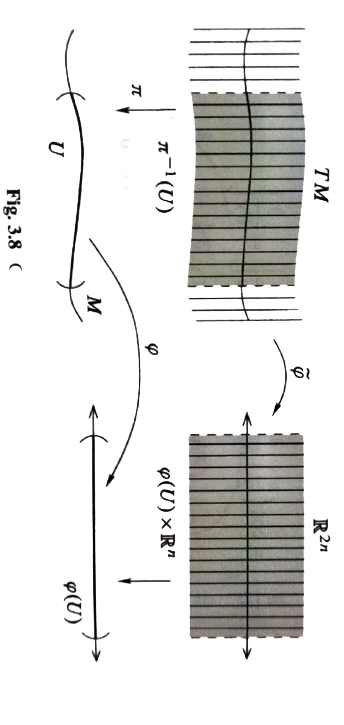
\includegraphics[angle=90,width=.7\linewidth]{figures/fog3.8.png}
        \caption{\textbf{Coordinate For the tangent bundle}}
        \label{fig:coordinate for tangent bundle}
    \end{figure}
    Its image set is $\varphi(U)\times\R^n$, which is an open subset of $\R^{2n}$. It is a bijection onto its image, because its inverse can be written explicitly as 
    \[\widetilde{\varphi}^{-1}(x^1,\cdots,x^n,v^1,\cdots,v^n)=v^i\frac{\partial}{\partial x^i}\bigg|_{\varphi^{-1}(x)}.\]
    Now suppose we are given two smooth charts $(U,\varphi)$ and $(V,\psi)$ for $M$, and let $(\pi^{-1}(U),\widetilde{\varphi}),(\pi^{-1}(V),\widetilde{\psi})$ be the corresponding charts on $TM$. The sets
    \begin{eq*}
        \widetilde{\varphi}\left(\pi^{-1}(U)\bigcap \pi^{-1}(V)\right)&=\varphi(U\bigcap V)\times \R^n \quad \textrm{and} \\ 
        \widetilde{\psi}\left(\pi^{-1}(U)\bigcap \pi^{-1}(V)\right)&=\psi(U\bigcap V)\times \R^n
    \end{eq*}
    are open in $\R^{2n}$, and the transition map $\widetilde{\psi}\circ \widetilde{\varphi}^{-1}\colon \varphi(U\bigcap V)\times \R^n\to \psi (U\bigcap V)\times \R^n$ can be written explicitly using 
    \begin{eq}
    \widetilde{v}^j=\frac{\partial \widetilde{x}^j}{\partial \widetilde{x}^i}(\hat{p})v^i
    \end{eq}
    as 
    \begin{eq*}
        \widetilde{\psi}&\circ \widetilde{\varphi}^{-1}(x^1,\cdots,x^n,v^1,\cdots,v^n) 
        =\left(\widetilde{x}^1 (x),\cdots,\widetilde{x}^n (x),\frac{\partial \widetilde{x}^1}{\partial \widetilde{x}^j}(x)v^j,\cdots,\frac{\partial \widetilde{x}^n}{\partial \widetilde{x}^j}(x)v^j\right)
    \end{eq*}
    This is clearly smooth.

    Choosing a countable cover $\{U_i\}$ of $M$ by smooth coordinate domains, we obtain a countable cover of $TM$ by coordinate domains $\{\pi^{-1}(U_i)\}$ satisfying conditions (i)-- (iv) of the smooth manifold chart lemma (Lemma 1.35). To check the Hausdorff condition (v), just note that any two points in the same fiber of $\pi$ lie in one chart, while if $(p,v)$ and $(q,w)$ lie in different fibers, there exists dijoint smooth coordinate domains $U,V$ for $M$ such that $p\in U$, and $q\in V$, and then $\pi^{-1}(U)$ and $\pi^{-1}(V)$ are disjoint coordinate neiborhoods containing $(p,v)$ and $(q,w)$, respectively.

    To see that $\pi$ is smooth, note that with respect to charts $(U,\varphi)$ for $M$ and $(\pi^{-1}(U),\widetilde{\varphi})$ for $TM$, its coordinate representation is $\pi(x,v)=x$.
\end{proof}
The coordinate $(x^i,v^i)$ given by \textbf{Eq~\eqref{eq:natural coordinates on TM}} are called \textbf{Natural Coordinates On $TM$}.
% \foottext{No matter how abstract any branch of mathematics is, it will one day be applied in the real world.}
% \footimage{terenceTao.jpg}

\begin{lem}
    $M_m$ 自然同构于 $(F_m/F_m^2)^*$.
\end{lem}
\begin{proof}
如果 $v \in M_m$, 那么由于求导运算的性质, $v$ 是 $F_m$ 上的线性函数且在 $F_m^2$ 上为零. 反过来, 如果 $l \in\left(F_m / F_m^2\right)^*$, 那么通过对 $\mathbf{f} \in \widetilde{F}_m$ 置 $v_l(\mathbf{f})=l(\{\mathbf{f}-\mathbf{f}(\mathbf{m})\})$ 来定义 $m$ 点的切向量 $v_l$ (其中, $\mathbf{f}(\mathbf{m})$ 表示取常数值 $\mathbf{f}(m)$ 的函数芽, \{\} 则用来表示 在 $F_m / F_m^2$ 中的陪集). $v_l$ 在 $\widetilde{F}_m$ 上的线性性质是明显的, 而它是一个求导运算是 因为
$$
\begin{aligned}
v_l(\mathbf{f} \quad \mathbf{g}) & =l(\{\mathbf{f} \mathbf{g}-\mathbf{f}(\mathbf{m}) \mathbf{g}(\mathbf{m})\}) \\
& =l(\{(\mathbf{f}-\mathbf{f}(\mathbf{m}))(\mathbf{g}-\mathbf{g}(\mathbf{m}))+\mathbf{f}(\mathbf{m})(\mathbf{g}-\mathbf{g}(\mathbf{m}))+(\mathbf{f}-\mathbf{f}(\mathbf{m})) \mathbf{g}(\mathbf{m})\}) \\
& =l(\{(\mathbf{f}-\mathbf{f}(\mathbf{m}))(\mathbf{g}-\mathbf{g}(\mathbf{m}))\})+\mathbf{f}(m) l(\{\mathbf{g}-\mathbf{g}(\mathbf{m})\})+\mathbf{g}(m) l(\{\mathbf{f}-\mathbf{f}(\mathbf{m})\}) \\
& =\mathbf{f}(m) v_{l}(\mathbf{g})+\mathbf{g}(m) v_{l} (\mathbf{f}) .
\end{aligned}
$$
从而得到 $M_m$ 到 $\left(F_m / F_m^2\right)^*$ 中的映射, 且反之亦然. 容易验证这些映射互逆, 因而 它们都是同构.
\end{proof}
\begin{thm}\label{thm:dimension equal}
$\dim\left(F_m / F_m^2\right)=\dim M$.
\end{thm}

证明是基于下列微积分的引理.
\begin{lem}
如果 $g$ 在 $\mathbb{R}^d$ 中包围 $p$ 点的一个凸开集 $U$ 上是 $C^k(k \geqslant 2)$ 类的, 那么对于 每个 $q \in U$,
\begin{multline}\label{eq:lem1.1.3}
g(q)= g(p)+\left.\sum_{i=1}^d \frac{\partial g}{\partial r_i}\right|_p\left(r_i(q)-r_i(p)\right) \\
 +\left.\sum_{i, j}\left(r_i(q)-r_i(p)\right)\left(r_j(q)-r_j(p)\right) \int_0^1(1-t) \frac{\partial^2 g}{\partial r_i \partial r_j}\right|_{(p+t(q-p))} \dd t .
\end{multline}
特别地, 若 $g \in C^{\infty}$, 那么\eqref{eq:lem1.1.3}~式中的第二个和式决定 $F_p^2$ 的一个元素, 因为积分 作为 $q$ 的一个函数是 $C^{\infty}$ 类的.
\end{lem}
\begin{proof}{(\textbf{定理~\ref{thm:dimension equal}~的证明})}

令 $(U, \varphi)$ 为 $m$ 点的坐标函数是 $x_1, \cdots, x_d ~(d=\dim M)$ 的坐标系. 令 $\mathbf{f} \in F_m$. 将\textbf{\eqref{eq:lem1.1.3}~式}应用于 $f \circ \varphi^{-1}$, 并且与 $\varphi$ 复合得到, 在 $m$ 的一个邻域上,
$$
f=\left.\sum_{i=1}^d \frac{\partial\left(f \circ \varphi^{-1}\right)}{\partial r_i}\right|_{\varphi(m)}\left(x_i-x_i(m)\right)+\sum_{i, j}\left(x_i-x_i(m)\right)\left(x_j-x_j(m)\right) h,
$$
其中, $h \in C^{\infty}$. 因而
$$
\mathbf{f}=\left.\sum_{i=1}^d \frac{\partial\left(f \circ \varphi^{-1}\right)}{\partial r_i}\right|_{\varphi(m)}\left(\mathbf{x}_i-\mathbf{x}_i(\mathbf{m})\right) \bmod F_m^2 .
$$
因此 $\left\{\left\{\mathbf{x}_i-\mathbf{x}_i(\mathbf{m})\right\}: i=1, \cdots, d\right\}$ 张成 $F_m / F_m^2$, 所以 $\operatorname{dim} F_m / F_m^2 \leqslant d$, 可以断言, 这些 元素是线性无关的. 因为假设
$$
\sum_{i=1}^d a_i\left(\mathbf{x}_i-\mathbf{x}_i(\mathbf{m})\right) \in F_m^2 .
$$
现在,
$$
\sum_{i=1}^d a_i\left(x_i-x_i(m)\right) \circ \varphi^{-1}=\sum_{i=1}^d a_i\left(r_i-r_i(\varphi(m))\right) .
$$
因而
$$
\sum_{i=1}^d a_i\left(\mathbf{r}_i-\mathbf{r}_i(\varphi(\mathbf{m}))\right) \in F_{\varphi(m)}^2 .
$$
但是这就蕴涵着, 对于 $j=1, \cdots, d$,
$$
\left.\frac{\partial}{\partial r_j}\right|_{\varphi(m)}\left(\sum a_i\left(r_i-r_i(\varphi(m))\right)\right)=0,
$$
而这又蕴涵着 $a_j$ 必然全为零.
\end{proof}

\begin{cor}
    $\dim M_m=\dim M$.
\end{cor}
\begin{thm}
    余切丛 $T^* M$ 是 $2n$ 维光滑流形.
\end{thm}
\begin{proof}
    我们可以讨论两个坐标卡 $\left(U, \phi ; x^i\right),\left(V, \varphi ; y^i\right)$ 相交部分的坐标变换,他们的基分别记为 $\left\{\left.d x^i\right|_p\right\},\left\{\left.d y^i\right|_p\right\} \subset T_p^* M$ ,将 $U$ 上的基用 $V$ 线性表出:
$$
\left.d x^i\right|_p=\left.a_k d y^k\right|_p, \quad \forall 1 \leq i \leq n .
$$
根据切空间的坐标变换,我们有:
$$
\left.\frac{\partial}{\partial y^l}\right|_p=\left.\frac{\partial x^j}{\partial y^l}\left(y_0\right) \frac{\partial}{\partial x^j}\right|_p,
$$
两边作用 $\left.d x^i\right|_p$ ,因为 $\left(d x^i,\left.\frac{\partial}{\partial x^j}\right|_p\right)=\delta_{i j}$ ,所以得到:
$$
d x^i\left(\left.\frac{\partial}{\partial y^l}\right|_p\right)=d x^i\left(\left.\frac{\partial x^j}{\partial y^l}\left(y_0\right) \frac{\partial}{\partial x^j}\right|_p\right)=\frac{\partial x^j}{\partial y^l} \delta_{i j}=\frac{\partial x^i}{\partial y^l}=a_k d y^k\left(\left.\frac{\partial}{\partial y^l}\right|_p\right)=a_l
$$
稍微把 $a$ 的指标从 $l$ 换为 $j$ ,就得到了对于余切空间的坐标变换公式:
$$
\left.d x^i\right|_p=\left.\frac{\partial x^i}{\partial y^j} d y^j\right|_p .
$$
接着再仿照上文中 $T M$ 是 $2 n$ 维流形的证明,就知道 $T^* M$ 仍然是 $2 n$ 维光滑流形,坐标卡的取法为:
$$
\left(\pi^{-1}(U), \varphi ; x^i\right): \varphi\left(\left.v_i d x^i\right|_p\right)=\left(x^1(p), \ldots, x^n(p), v_1, \ldots, v_n\right)
$$
对两个坐标卡 $\left(\pi^{-1}(U), \varphi ; x^i\right),\left(\pi^{-1}(V), \psi ; y^i\right)$ 转移函数为:
$$
\psi \circ \varphi^{-1}\left(x^1, \ldots, x^n, v_1, \ldots, v_n\right)=\left(y^1(x), \ldots, y^n(x), \frac{\partial x^1}{\partial y^j} v_j, \ldots, \frac{\partial x^n}{\partial y^j} v_j\right)
$$
第二可数以及Hausdorff亦可以验证。

更进一步,仿照$TM$是可定向流形,我们也可以证明 $T^* M$ 为可定向流形,其中关键一步是在考虑转移函数的雅可比时,根据余切丛上的坐标变换,后 $n$ 个分量的雅可比恰好是前 $n$ 个分量雅可比的倒数,所以转移函数的雅可比恒为 $1$,因此可定向。
\end{proof}
\section{Frobenius定理}\label{thm:frobenius 1 denmension}
\begin{thm}[一维情形Frobenius定理 (归纳法的第一步)]
    令 $m\in M^d$, 且令 $X$ 是 $M$ 上的一个光滑向量场使得 $X(m)\neq 0$,那么在 $m$ 的一个邻域上存在一个以 $x_1,\cdots,x_d$ 为坐标函数的坐标系使得
    \begin{equation}
        X\big|_U =\frac{\partial}{\partial x_1}\bigg|_U.
    \end{equation}
\end{thm}
\begin{proof}
    选取一个中心在 $m$ 点、坐标函数为 $y_1, \cdots, y_d$ 的坐标系 $(V, \tau)$ 使得
\begin{equation}\label{eq:1.5}
X_m=\left.\frac{\partial}{\partial y_1}\right|_m .
\end{equation}
从下述命题\ref{prop:1.48 (d)}
\begin{prop}\label{prop:1.48 (d)}
    对于每个 $m\in M$, 存在 $m$ 的一个开邻域 $V$和一个 $\varepsilon>0$,使得从 $(-\varepsilon,\varepsilon)\times V$到 $M$的映射
    \begin{equation}
        (t,p)\mapsto X_t (p)
    \end{equation}
    是有定义的而且是 $C^\infty$的.
\end{prop}
可知, 存在一个 $\varepsilon>0$ 和 $\mathbb{R}^{d-1}$ 中原点的一个邻域 $W$ 使得映射
$$
\sigma\left(t, a_2, \cdots, a_d\right)=X_t\left(\tau^{-1}\left(0, a_2, \cdots, a_d\right)\right)
$$
对于 $\left(t, a_2, \cdots, a_d\right) \in(-\varepsilon, \varepsilon) \times W \subset \mathbb{R}^d$ 是完全确定的而且是光滑的, 于是 $\sigma$ 在原点是 非奇异的, 因为
$$
\mathrm{d} \sigma\left(\left.\frac{\partial}{\partial r_1}\right|_0\right)=X_m=\left.\frac{\partial}{\partial y_1}\right|_m \quad \text { 和 } \mathrm{d} \sigma\left(\left.\frac{\partial}{\partial r_i}\right|_0\right)=\left.\frac{\partial}{\partial y_i}\right|_m \quad(i \geqslant 2) \text {. }
$$
因而由命题\ref{prop:1.30系a}
\begin{prop}\label{prop:1.30系a}
    假设 $\psi\colon M\to N$ 是 $C^\infty$映射, $m\in M$,并且 $\dd \psi\colon M_m\to N_{\psi(m)}$是一个同构,那么存在 $m$的一个邻域 $U$使得 $\psi\colon U\to \psi(U)$是到 $N$ 中开集 $\psi(U)$上的一个微分同胚.
\end{prop}
可知 $\varphi=\sigma^{-1}$ 是 $m$ 的某个邻域 $U$ 上的坐标映射. 令 $x_1, \cdots, x_d$ 表示坐 标系 $(U, \varphi)$ 的坐标函数, 那么由于
$$
\mathrm{d} \sigma\left(\left.\frac{\partial}{\partial r_1}\right|_{\left(t, a_2, \cdots, a_d\right)}\right)=X_{\sigma\left(t, a_2, \cdots, a_d\right)},
$$
所以有
$$
\left.X\right|_U=\left.\frac{\partial}{\partial x_1}\right|_U .
$$
\end{proof}
\begin{thm}[Frobenius定理]\label{thm: Frobenius}
    令 $\mathscr{D}$ 是 $M^d$ 上的一个 $c$ 维 $C^{\infty}$  对合分布. 令 $m \in M$, 那 么存在 $\mathscr{D}$ 的一个过 $m$ 的积分流形. 实际上, 存在一个以 $m$ 为中心, 以 $x_1, \cdots, x_d$ 为 坐标函数的立方体坐标系 $(U, \varphi)$ 使得片
    \begin{equation}
        \label{eq:1.7}
        x_i= \text{常数, 所有} ~i \in\{c+1, \cdots, d\}
    \end{equation}
都是 $\mathscr{D}$ 的积分流形. 而且如果 $(N, \psi)$ 是 $\mathscr{D}$ 的连通积分流形使得 $\psi(N) \subset U$, 那么 $\psi(N)$ 位于这些片之一中.
\end{thm}
\begin{proof}
用关于 $c$ 的归纳法来证明定理的存在性部分. 对于 $c=1$ 的情况, 选取 一个位于 $\mathscr{D}$ 中的、在 $m$ 的一个开邻域上定义的向量场 $X$ 使得 $X(m) \neq 0$, 那么由\textbf{定理 ~\ref{thm:frobenius 1 denmension}}~产生 $m$ 点的一个坐标系 $(U, \varphi)$, 它可以取为中心的立方体的, 使得 $\left.X\right|_U=\frac{\partial}{\partial x_1}$. 因此定理对于 $c=1$ 成立.

现在设对于 $c-1$ 定理成立, 证明它对于 $c$ 维分布 $\mathscr{D}$ 成立. 因为 $\mathscr{D}$ 是光滑的, 所 以在 $m$ 的一个邻域 $\tilde{V}$ 上存在张成 $\mathscr{D}$ 的光滑向量场 $X_1, \cdots, X_c$. 由\textbf{定理 ~\ref{thm:frobenius 1 denmension}}, 存在以 $m$ 为中心并且适合 $V \subset \tilde{V}$ 的坐标系 $\left(V, y_1, \cdots, y_d\right)$ 使得
\begin{equation}
    \label{eq:1.8}
    \left.X_1\right|_V=\frac{\partial}{\partial y_1} .
\end{equation}
在 $V$ 上, 令
\begin{equation}
    \label{eq:1.9}
    \left\{\begin{array}{l}
Y_1=X_1, \\
Y_i=X_i-X_i\left(y_1\right) X_1 \quad(i=2, \cdots, c),
\end{array}\right.
\end{equation}
那么向量场 $Y_1, \cdots, Y_c$ 是在 $V$ 中张成 $\mathscr{D}$ 的独立 $C^{\infty}$ 向量场. 令 $S$ 是片 $y_1=0$, 并且令
\begin{equation}\label{eq:1.10}
    Z_i=Y_i |_S\quad (i=2,\cdots,c).
\end{equation}
那么因为 \eqref{eq:1.8}和\eqref{eq:1.9}蕴涵着
\begin{equation}
    \label{eq:1.11}
    Y_i\left(y_1\right)=0 \quad(i=2, \cdots, c),
\end{equation}

所以 $Z_i$ 实际上是 $S$ 上的向量场, 即当 $q \in S$ 时, $Z_i(q) \in S_q . Z_i$ 张成 $S$ 上的一个 $c-1$ 维 光滑分布. 可以断言这个分布是对合的. 实际上, $Z_i$ 与 $Y_i$ 是 $i$ 相关的 $(i$ 是 $S$ 在 $M$ 中 的包含映射), 因此由\textbf{命题~\ref{prop:relevant}}, $Z_i$ 的 Lie 括号与 $Y_i$ 的 Lie 括号也是 $i$ 相关的. 但是 $\left[Y_{i,} Y_j\right](i, j \geqslant 2)$ 没有沿 $Y_1$ 方向的分量(应用于 $y_1$ 等于 0 ). 因此存在 $C^{\infty}$ 函数 $c_{i j}$, 使得 在 $V$ 上
\begin{equation}
    \label{eq:1.12}
    \left[Y_i, Y_j\right]=\sum_{k=2}^c c_{i j k} Y_k,
\end{equation}
因而
\begin{equation}
    \label{eq:1.13}
    \left[Z_i, Z_j\right]=\left.\sum_{k=2}^c c_{i j k}\right|_S Z_k .
\end{equation}
这证明 $S$ 上的分布是对合的. 由归纳假设, 在 $S$ 中存在 $m$ 的某个邻域上的中心坐 标系 $w_2, \cdots, w_d$ 使得对所有 $i \in\{c+1, \cdots, d\}$, 由 $w_i=$ 常数定义的片恰好是这个邻域上 由 $Z_2, \cdots, Z_c$ 张成的分布的积分流形.
函数
\begin{equation}
    \label{eq:1.14}
    \left\{\begin{array}{l}
x_1=y_1, \\
x_j=w_j \circ \pi \quad(j=2, \cdots, d)
\end{array}\right.
\end{equation}
(其中, $\pi: V \rightarrow S$ 是 $y$ 坐标系中的自然射影)于 $m$ 在 $M$ 中的某个邻域上有定义, 它
们在 $m$ 点是独立的, 而且它们在 $m$ 点全为零. 因而在 $m$ 的一个适当邻域 $U$ 上有 一个以 $x_1, \cdots, x_d$ 为坐标函数的中心立方体坐标系 $(U, \varphi)$. 现在证明在 $U$ 上,
\begin{equation}
    \label{eq:1.15}
    Y_i\left(x_{c+r}\right) \equiv 0 \quad(i=1, \cdots, c ; r=1, \cdots, d-c) .
\end{equation}
由此可知, 向量场 $\frac{\partial}{\partial x_i}, \cdots, \frac{\partial}{\partial x_c}$ 在 $U$ 的每一点构成 $\mathscr{D}$ 的基, 因而片\eqref{eq:1.7}是 $\mathscr{D}$ 的积分流形.
为了证明 \eqref{eq:1.15}, 我们首先注意到 \eqref{eq:1.14} 蕴涵着在 $U$ 上
\begin{equation}
    \label{eq:1.16}
    \frac{\partial x_j}{\partial y_1}= \begin{cases}1 & (j=1), \\ 0 & (j=2, \cdots, d),\end{cases}
\end{equation}
从而\eqref{eq:1.8}, \eqref{eq:1.9}及 \eqref{eq:1.16}蕴涵着在 $U$ 上
\begin{equation}
    \label{eq:1.17}
    Y_1=\frac{\partial}{\partial x_1},
\end{equation}
所以\eqref{eq:1.15}对 $i=1$ 肯定成立. 现在令 $i \in\{2, \cdots, c\}, r \in\{1, \cdots, d-c\}$, 那么由\eqref{eq:1.17}, 有
\begin{equation}
    \label{eq:1.18}
    \frac{\partial}{\partial x_1}\left(Y_i\left(x_{c+r}\right)\right)=Y_1\left(Y_i\left(x_{c+r}\right)\right)=\left[Y_1, Y_i\right]\left(x_{c+r}\right) .
\end{equation}
$\mathscr{D}$ 的对合性蕴涵着有函数 $c_{i k}$, 使得
\begin{equation}
    \label{eq:1.19}
    \left[Y_1, Y_i\right]=\sum_{k=1}^c c_{i k} Y_k .
\end{equation}
利用\eqref{eq:1.19}, 则\eqref{eq:1.18}变为
\begin{equation}\label{eq:1.20}
    \frac{\partial}{\partial x_1}(Y_i (x_{c+r}))=\sum_{k=2}^c c_{ik} Y_k (x_{c+k}) \quad (i=2,\cdots,c; r=1,\cdots,d-c).
\end{equation}
固定 $U$ 的形如 $x_2=$ 常数, $\cdots, x_d=$ 常数的一个片. 在这样一个片上, $Y_i\left(x_{c+r}\right)$ 仅为 $x_1$ 的 函数, 而且 \eqref{eq:1.20}变为关于 $x_1$ 的 $c-1$ 维齐次线性微分方程组. 这样的微分方程组对 于给定的初始值有唯一的解. 因为方程组是齐次的, 所以零函数是一个解. 但 是每个这样的片在 $S \cap U$ 中有唯一一个点, 而且在 $S \cap U$ 上,
\begin{equation}
    \label{eq:1.21}
Y_i\left(x_{c+r}\right)=Z_i\left(w_{c+r}\right)=0 \quad(i=2, \cdots, c) .
\end{equation}
第一个等式从\eqref{eq:1.10}和\eqref{eq:1.14}得出; 第二个等式可从下列事实得出: $S$ 上由 $Z_i$ 决定的分布的积分流形是由 $w$ 坐标系中的适当的片给出的. 从\eqref{eq:1.20}和\eqref{eq:1.21}得知, 函数 $Y_i\left(x_{c+r}\right)$ 在 $U$ 上必然恒为零, 因而 \eqref{eq:1.15}成立, 于是归纳步裛完成.
最后设 $(N, \psi)$ 是 $\mathscr{D}$ 的一个连通积分流形并且使得 $\psi(N) \subset U$. 令 $\pi$ 是 $\mathbb{R}^d$ 到最后 $d-c$ 个坐标上的射影, 那么 $\mathscr{D}$ 中的向量被 $\mathrm{d}(\pi \circ \varphi)$ 零化. 因而对于每个 $n \in N$,
$$
\left.\mathrm{d}(\pi \circ \varphi \circ \psi)\right|_n \equiv 0 .
$$
由下面的定理\ref{thm:1.24},
\begin{thm}\label{thm:1.24}
    令 $\psi$ 是从连通流形 $M$到 流形 $N$的一个光滑映射.如果对每个 $m\in M,\dd \psi_m\equiv 0$,那么 $\psi$必是一个常值映射.
\end{thm}
可知 $\pi \circ \varphi \circ \psi$ 是一个常值映射, 因为 $N$ 是连通的. 从而 $\psi(N)$ 包含在由
\begin{equation}
    \dd \psi(N_n)=\mathscr{D}(\psi(n)).
\end{equation}
所表示的一个片中.
\end{proof}

\begin{remark}
 Frobenius(弗罗贝尼乌斯)定理的经典形式显得与 $1.60$ 节中的形式很不相同. 经典的 Frobenius 定理可以表述如下:
令 $U$ 和 $V$ 分别为 $\mathbb{R}^m$ 和 $\mathbb{R}^n$ 中的开集. 在 $\mathbb{R}^m$ 上使用坐标 $r_1, \cdots, r_m$ 而在 $\mathbb{R}^n$ 上使 用坐标 $s_1, \cdots, s_n$. 令
\begin{equation}
    \label{eq:1.22}
    b: U \times V \rightarrow M(n, m)
\end{equation}
是从 $U \times V$ 到所有 $n \times m$ 实矩阵的集合中的一个 $C^{\infty}$ 映射, 令 $\left(r_0, s_0\right) \in U \times V$. 如 果在 $U \times V$ 上,
\begin{equation}
    \label{eq:1.23}
    \begin{gathered}
\frac{\partial b_{i \beta}}{\partial r_\gamma}-\frac{\partial b_{i \gamma}}{\partial r_\beta}+\sum_{j=1}^n\left(\frac{\partial b_{i \beta}}{\partial s_j} b_{j \gamma}-\frac{\partial b_{i \gamma}}{\partial s_j} b_{j \beta}\right)=0 \\
(i=1, \cdots, n ; \gamma, \beta=1, \cdots, m),
\end{gathered}
\end{equation}
那么存在 $r_0$ 在 $U$ 中的邻域 $U_0$ 和 $s_0$ 在 $V$ 中的邻域 $V_0$ 以及唯一的一个 $C^{\infty}$ 映射
\begin{equation}
    \label{eq:1.24}
    \alpha: U_0 \times V_0 \rightarrow V
\end{equation}
使得若
\begin{equation*}
    \alpha_s (r) =\alpha (r,s)\quad (r\in U_0,s\in V_0),
\end{equation*}
则对所有 $(r,s)\in U_0\times V_0$,
\begin{equation}\label{eq:1.25}
    \begin{cases}
        \alpha_s (r_0)=s,\\ 
        \dd \alpha_s|_r=b(r,\alpha(r,s)).
    \end{cases}
\end{equation}
方程\eqref{eq:1.24}是全微分方程. 在 \eqref{eq:1.22} 中说明映射的微分应像一个图函数, 并且在\eqref{eq:1.23}中得到带有特定初始条件的这样一个映射存在的充分必要条件. 可以证明这 种形式等价于定理 1.60. 例如, 若从 $M^d$ 上的一个对合的 $c$ 维 $C^{\infty}$ 分布 $\mathscr{D}$ 和一个点 $m \in M$ 开始, 则能够从经典形式得出定理 $1.60$ 如下: 首先选取 $m$ 点的一个坐标系 $(W, \tau)$, 以 $y_1, \cdots, y_d$ 为坐标函数且适合 $\tau(W)=U \times V \subset \mathbb{R}^c \times \mathbb{R}^{d-c}$, 而且在 $U \times V$ 上存在 $C^{\infty}$ 函数 $f_{j i}(i=1, \cdots, c ; j=1, \cdots, d-c)$ 使得向量场
\begin{equation}
    \label{eq:1.26}
    Y_i=\frac{\partial}{\partial y_i}+\sum_{j=1}^{d-c} f_{j i} \circ \tau \frac{\partial}{\partial y_{c+j}} \quad(i=1, \cdots, c)
\end{equation}
在 $W$ 上张成 $\mathscr{D}$, 那么可以像在\eqref{eq:1.22}中那样通过置
\begin{equation}
    \label{eq:1.27}
    b(r, s)=\left\{f_{j i}(r, s)\right\}
\end{equation}
来定义一个映射 $b$. 结果, $\mathscr{D}$ 的对合性蕴涵着 \eqref{eq:1.23}被满足, 而且从映射 $\alpha$ 就能得到所要求的坐标系 $1.60(1)$. 反过来也能用类似的方法从 \ref{thm: Frobenius}得出定理的经典形式.


第 2 章将给出以微分形式和微分理想表述的 Frobenius 定理的另一种形式. 
\end{remark}
\clearpage
\begin{thm}[Frobenius定理用微分形式与微分理想表示的形式]
    令 $\mathscr{T} \subset E^*(M)$ 是一个由 $d-p$ 个独立 $1$ 形式局部生成的微分理想. 令 $m \in M$, 那么经过 $m$ 点存在唯一的一个极大连通积分流形, 并且这个积分流形是 $p$ 维的.
\end{thm}
\section{测试定理样式}
\begin{theorem}[Frobenius定理用微分形式与微分理想表示的形式][thm:test thm]
    令 $\mathscr{T} \subset E^*(M)$ 是一个由 $d-p$ 个独立 $1$ 形式局部生成的微分理想. 令 $m \in M$, 那么经过 $m$ 点存在唯一的一个极大连通积分流形, 并且这个积分流形是 $p$ 维的.
\end{theorem}

\begin{lemma}[Frobenius定理用微分形式与微分理想表示的形式][thm:test lem]
    令 $\mathscr{T} \subset E^*(M)$ 是一个由 $d-p$ 个独立 $1$ 形式局部生成的微分理想. 令 $m \in M$, 那么经过 $m$ 点存在唯一的一个极大连通积分流形, 并且这个积分流形是 $p$ 维的.
\end{lemma}

\begin{definition}[Frobenius定理用微分形式与微分理想表示的形式][thm:test def]
    令 $\mathscr{T} \subset E^*(M)$ 是一个由 $d-p$ 个独立 $1$ 形式局部生成的微分理想. 令 $m \in M$, 那么经过 $m$ 点存在唯一的一个极大连通积分流形, 并且这个积分流形是 $p$ 维的.
\end{definition}

\begin{proposition}[Frobenius定理用微分形式与微分理想表示的形式][thm:test prop]
    令 $\mathscr{T} \subset E^*(M)$ 是一个由 $d-p$ 个独立 $1$ 形式局部生成的微分理想. 令 $m \in M$, 那么经过 $m$ 点存在唯一的一个极大连通积分流形, 并且这个积分流形是 $p$ 维的.
\end{proposition}

\begin{example}[Frobenius定理用微分形式与微分理想表示的形式][thm:test example]
    令 $\mathscr{T} \subset E^*(M)$ 是一个由 $d-p$ 个独立 $1$ 形式局部生成的微分理想. 令 $m \in M$, 那么经过 $m$ 点存在唯一的一个极大连通积分流形, 并且这个积分流形是 $p$ 维的.
\end{example}

\begin{corollary}[Frobenius定理用微分形式与微分理想表示的形式][cor:test thm]
    令 $\mathscr{T} \subset E^*(M)$ 是一个由 $d-p$ 个独立 $1$ 形式局部生成的微分理想. 令 $m \in M$, 那么经过 $m$ 点存在唯一的一个极大连通积分流形, 并且这个积分流形是 $p$ 维的.
\end{corollary}
\clearpage
\begin{fancybox}
    令 $\mathscr{T} \subset E^*(M)$ 是一个由 $d-p$ 个独立 $1$ 形式局部生成的微分理想. 令 $m \in M$, 那么经过 $m$ 点存在唯一的一个极大连通积分流形, 并且这个积分流形是 $p$ 维的.
\end{fancybox}

\begin{solution}
testing
\end{solution}


































































































